% THIS IS A LATEX TEMPLATE FILE FOR PAPERS INCLUDED IN THE
% *Anthology of Computers and the Humanities*. ADD THE OPTION
% 'final' WHEN CREATING THE FINAL VERSION OF THE PAPER. 
% DO NOT change the documentclass
\documentclass[final]{anthology-ch} % for the final version
%\documentclass{anthology-ch}         % for the submission

% LOAD LaTeX PACKAGES
\usepackage{booktabs}
\usepackage{graphicx}
% ADD your own packages using \usepackage{}

% TITLE OF THE SUBMISSION
% Change this to the name of your submission
\title{Clouds for Crowds - Implementing Federated AAI for the Digital Humanities}

% AUTHOR AND AFFILIATION INFORMATION
% For each author, include a new call to the \author command, with
% the numbers in brackets indicating the associated affiliations 
% (next section) and ORCID-ID for each author.  
\author[1]{Tibor K\'alm\'an}[
  orcid=0000-0001-5194-5053
]

\author[2]{Sally Chambers}[
  orcid=0000-0002-2430-475X
]

% While we encourage including ORCID-IDs for all authors, you can
% include authors that do not have one by definining an empty ID.
\author[3]{Peter Gietz}[
  orcid=0000-0002-8310-2015
]

% There should be one call to \affiliation for each affiliation of
% the authors. Multiple affiliations can be given to each author
% and an affiliation can be given to multiple authors. 
\affiliation{1}{GWDG, G\"ottingen, Germany}
\affiliation{2}{DARIAH, Paris, France}
\affiliation{3}{DAASI International, T\"ubingen, Germany}

% KEYWORDS
% Provide one or more keywords or key phrases seperated by commas
% using the following command
\keywords{DARIAH AAI, AARC TREE, Authentication and Authorisation Infrastructure, AAI, AARC Blueprint Architecture}

% METADATA FOR THE PUBLICATION
% This will be filled in when the document is published; the values can
% be kept as their defaults when the file is submitted
\pubyear{2025}
\pubvolume{2}
\pagestart{32}
\pageend{37}
\conferencename{Digital Humanities Tech Symposium 2025}
\conferenceeditors{Julia Damerow and Rebecca Sutton Koeser}
\doi{10.63744/a9oVejGuN3UN}  

\addbibresource{bibliography.bib}

%%%%%%%%%%%%%%%%%%%%%%%%%%%%%%%%%%%%%%%%%%%%%%%%%%%%%%%%%%%%%%%%%%%%%%%%%%%
% HERE IS THE START OF THE TEXT
\begin{document}

\maketitle


\begin{abstract}
Technology has been inherent to the digital humanities from the outset. However, with the increase in data-driven research, Research Infrastructures (RI) such as DARIAH (Digital Research Infrastructure for the Arts and Humanities) need to ensure secure access to the data, tools and workflows they offer. Furthermore, collaboration with other RIs through initiatives such as OSCARS (Open Science Clusters’s Action for Research and Society) and compatibility with the European Open Science Cloud (EOSC) are becoming increasingly important. It is within this context that this article aims to highlight the necessity and advantages of implementing federated identity management and authorisation. It describes the technological background of such an Authentication and Authorisation Infrastructure (AAI) solution for the digital humanities. Finally, it motivates the DHTech community to adopt the AARC Blueprint Architecture supported by a Compendium being developed in the context of the AARC-TREE project. 
\end{abstract}



\section{Research Infrastructure for the Arts and Humanities} 

DARIAH (Digital Research Infrastructure for the Arts and Humanities)~\cite{web_dariah} is a European research infrastructure that provides a platform for researchers in the arts and humanities to access, share, and preserve digital resources and tools~\cite{sshoc_marketplace}. DARIAH aims to enhance and support digitally-enabled research in the arts and humanities, fostering collaboration, innovation and knowledge-sharing across disciplines and borders~\cite{chambers_2025_14881627}. The infrastructure offers a range of services, including repositories, virtual research environments, and authentication and authorisation mechanisms, to support the research lifecycle and facilitate the creation, publication, and preservation of digital scholarship. By providing a shared infrastructure and community-driven approach, DARIAH enables researchers to work together more effectively, leveraging digital methods and tools to advance our understanding of human culture and society. The technical foundation for this shared infrastructure is provided by the DARIAH AAI (Authentication and Authorisation Infrastructure)~.

This paper provides an overview of the DARIAH AAI from the authors' perspective. One author is one of the developers of the DARIAH AAI, one is responsible for its current operation, and one holds a management position within DARIAH. This paper provides insights into the technical aspects of the DARIAH infrastructure with the goal to encourage others to build on top of DARIAH AAI by following AAI best practices, and to showcase a sustainable integration pathway for DH services and DH communities into the global research infrastructure landscape.


\section{AAI for DARIAH}

The DARIAH AAI \cite{web_dariahaai} is a federated identity management system designed to facilitate secure and seamless access to data, tools and workflows for researchers in the humanities and arts. By leveraging federated authentication and authorisation, service providers can benefit from improved security, reduced administrative burdens, and enhanced user experience. Federated authentication allows users to access multiple services with a single set of credentials (e.g. their home institution login), eliminating the need for multiple usernames and passwords. This approach also enables service providers to outsource identity management to trusted identity providers, reducing the risk of password breaches and minimising the administrative effort required to manage user accounts. Furthermore, federated authorisation enables fine-grained access control, allowing developers to define and enforce precise access policies based on user attributes, group memberships and roles. From the user perspective, the DARIAH AAI also allows for single sign-on (SSO), i.e. the user authenticates once after connecting to a first application and is then automatically authenticated for all other federated applications they want to use the same day. 
By adopting the DARIAH AAI, service providers and developers can focus on delivering high-quality services to their users, while relying on a robust and scalable infrastructure to manage authentication and authorisation.



\section{Technological Background}

The technological background of DARIAH AAI is provided using established technologies and standardised protocols for federated identity management, as summarised below. More background information can be found in Chapter 3.3.3, \textit{Access control to research data in the frame of FAIR principles and open access} \cite{erzsebet_toth_czifra_2023_8059626}.

\textbf{SAML (Security Assertion Markup Language).} The DARIAH AAI uses SAML as the primary protocol for exchanging authentication and authorisation information between identity providers and service providers. SAML allows for the secure exchange of user attributes and authentication statements between parties.

\textbf{OpenID Connect (OIDC).} In addition to SAML, the DARIAH AAI also supports OIDC, an authentication protocol built on top of the OAuth 2.0 framework. OIDC provides a simpler and more lightweight alternative to SAML for authentication and authorisation.

\textbf{OAuth 2.0.} The DARIAH AAI also supports OAuth 2.0 as the authorisation framework for managing access to protected resources. OAuth 2.0 provides a standardised mechanism for clients to request access to resources on behalf of the user.

\textbf{Shibboleth and SimpleSAMLphp.} The DARIAH AAI is based on the Shibboleth and simpleSAMLphp open source software systems, which provide a robust and scalable framework for managing identity federation. Both products support SAML and OIDC, and can provide a single sign-on (SSO) experience across both protocols.

\textbf{Role-based Access Control (RBAC).} The DARIAH AAI implements RBAC as a policy-based approach to access control. It allows for fine-grained access control decisions based on user roles, affiliations and permissions.
    
\textbf{LDAP (Lightweight Directory Access Protocol).} The DARIAH AAI uses LDAP as a directory service for storing and managing user attributes and identity information, as well as group memberships and roles.

\textbf{SP/IdP Proxy (Service Provider / Identity Provider Proxy).} DARIAH’s SP/IdP proxy simplifies the connection of services and identity sources to the infrastructure. This mechanism enables  any DARIAH related attributes (e.g. member of a specific research project), to be provided, in addition to the attributes provided by the home organisation.

The DARIAH AAI is designed to support federation, which means that it allows multiple identity providers and service providers to participate in the infrastructure. This enables users to access multiple services with a single set of credentials, while also allowing service providers to outsource identity management to trusted identity providers. It interconnects, for example, with eduGAIN~\cite{web_eduGAIN}, the interfederation of national research federations world-wide. Thus a researcher from a country that is part of the interfederation can access federated services world-wide by using the credentials managed by their home organisation.

Figure~\ref{fig:dariahaai1} depicts the DARIAH AAI architecture.
%
\begin{figure}[t!]
  \centering
  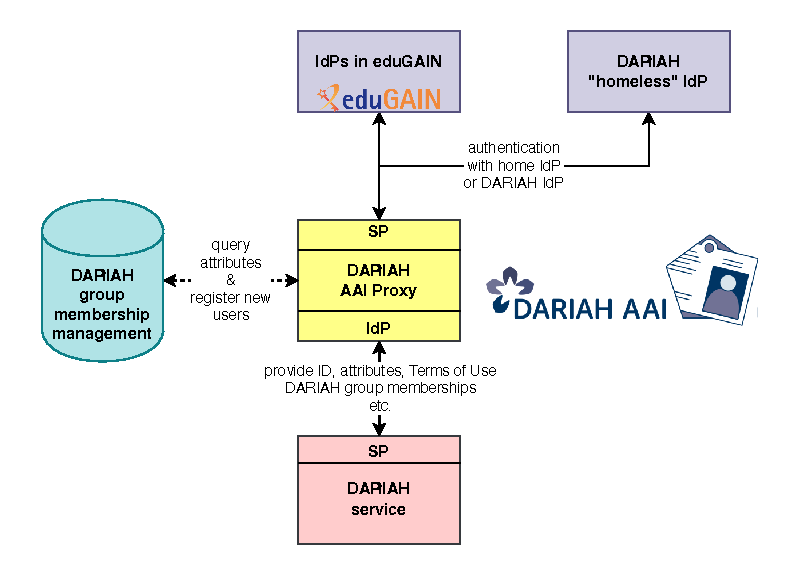
\includegraphics[width=0.7\linewidth]{figures/Figure_dariahaai1-v2.pdf}
  \caption{The Architecture of the DARIAH Authentication and Authorisation Infrastructure.}
  \label{fig:dariahaai1}
\end{figure}
%
The DARIAH SP/IdP Proxy allows authentication for (1) users from every IdPs interfederated in eduGAIN, as well as for (2) so-called “homeless” users from the DARIAH “homeless” IdP, where any humanities researcher can register for an account including independent researchers without an institutional affiliation. 
For users of both categories ("eduGAIN" or "homeless"), DARIAH-specific rights and privileges can be managed with the DARIAH group membership management. This enables the proxy to transfer user attributes from the IdP where the authentication took place, as well as membership attributes from the DARIAH virtual organisation to the DARIAH services.

By leveraging the above mentioned standard technologies and protocols, the DARIAH AAI provides a robust, scalable and secure system for managing identity and access control in the context of the research landscape. The majority of the design decisions made for the DARIAH AAI are compliant with the globally recognised AARC Blueprint Architecture.



\section{AARC Blueprint Architecture}

The AARC (Authentication and Authorisation for Research and Collaboration) Blueprint Architecture~\cite{aarc_community_members_2019_3672785} is a comprehensive framework for designing and implementing federated authentication and authorisation infrastructures for research communities. Developed through three phases of AARC projects~\cite{web_AARC}, the Blueprint provides a set of guidelines, policies and architectures for building scalable and secure identity management systems. DARIAH AAI implements the main components of AARC, including: \textbf{(1) Policy Framework}, which defines the rules and guidelines for identity management and access control; \textbf{(2) Proxy-based Architecture}, which outlines the technical design and components of the infrastructure; \textbf{(3) Standards and Protocols}, which specify the interoperability standards for identity federation and attribute-based access control; and \textbf{(4) Governance}, which establishes the organisational and operational structures for managing the infrastructure. 
By following the AARC Blueprint, research organisations and communities can establish robust and trustworthy identity management systems (like DARIAH AAI), to enable secure and seamless collaboration and access to shared resources and services. 

The current AARC TREE project (AARC Technical Revision to Enhance Effectiveness)~\cite{web_aarc_tree} drives the next phase of integration for research infrastructures. It expands federated access management to integrate user-centred technologies and access to federated data and services (authorisation), as well as defining common strategies for the development, deployment and sustainability of AAIs.
A key aim of the AARC TREE project is to foster the uptake of the AARC Blueprint Architecture and Guidelines by research infrastructures and their communities such as DARIAH. This work is supported by the development of a Compendium of AARC best practices and recommendations for a common long-term strategy for AAI services in pan-European Research Infrastructures in Europe. Furthermore, this work will lay the foundations for ensuring that the AAIs are compatible with the European Open Science Cloud. 



\section{EOSC and pan-European e-Infrastructures}
 
The European Open Science Cloud (EOSC) \cite{web_eosc} is a virtual environment that brings together research communities, data repositories, and service providers to enable seamless access to research data, services, and resources. 
The EOSC Federation~\cite{eosc_association_2025_14999577} enables the distributed management of such data, knowledge and resources for European research, fostering collaboration, innovation, and the uptake of open science.

At the heart of the EOSC Federation are the EOSC Nodes, which are national or thematic hubs that provide access to research services, data, and resources. EOSC Nodes are responsible for aggregating and providing services, data, and resources from their respective domains, making them available to the broader research community through the EOSC Federation. Each Node acts as a gateway to the EOSC, providing a single point of access to a wide range of research services, including data repositories, computing resources, and software tools. By connecting to the EOSC Federation through the Nodes, researchers can access a vast array of resources and services, facilitating collaboration, data sharing, and innovation across disciplines and borders. The EOSC Nodes play a crucial role in realising the vision of the EOSC, enabling the creation of a unified, open, and accessible research environment for European scientists. The basis of the EOSC Federation is the EOSC AAI as described in \cite{kanellopoulos_2025_15388270}, which interoperates with the DARIAH AAI.

\begin{figure}[t!]
  \centering
  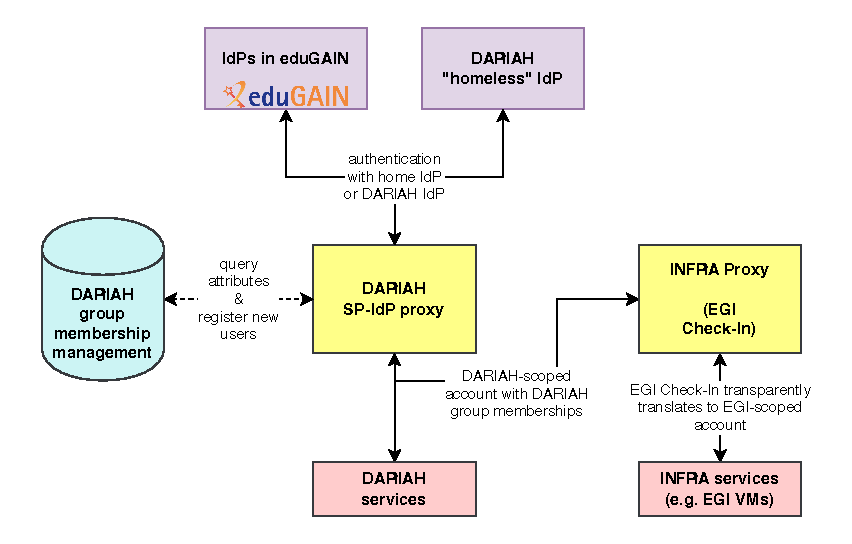
\includegraphics[width=0.7\linewidth]{figures/Figure_dariahaai2-v2.pdf}
  \caption{Interoperation between DARIAH-AAI and Services of a Research Infrastructure.}
  \label{fig:dariahaai2}
\end{figure}

DARIAH AAI's interoperability with pan-European e-infrastructures 
has already been successfully validated by various proof of concepts implementations (PoC).
For instance, \cite{dariah_poc} showcases how 
DARIAH-AAI users could access services from other e-infrastructures, by using the DARIAH AAI proxy as presented in the Figure~\ref{fig:dariahaai2}.
The Figure also shows how the DARIAH-AAI proxy provides a powerful layer of identity harmonisation (account linking capabilities) by interacting with other infrastructure proxies (like EGI's Check-In service or the EOSC EU Node's MyAccessID service).

With the European Open Science Cloud entering its build-up phase, 
such federated access is crucial for enabling humanities researchers to connect to the wealth of data, services and resources available.
Based on these undertakings it is now possible to productively login to the EOSC EU Node, via the DARIAH AAI.

\section{Conclusion}

Robust federated identity management and authorisation for research infrastructures such as DARIAH is becoming increasingly essential. By ensuring that the DARIAH-AAI is compatible with the AARC Blueprint Architecture and related initiatives such as EOSC, its adoption not only helps to simplify the management of access control and authorisation for DH service providers, but also reduces administrative burdens and most importantly, improves the overall user experience for researchers in the humanities and arts. 


\section*{Acknowledgments}

This work was partly funded by the European Union (AARC TREE project, grant agreement no. 101131237).
We would also like to acknowledge the support and contributions of the AARC community, and we are grateful for the feedback provided by the DARIAH community.



% Print the biblography at the end. Keep this line after the main text of your paper, and before an appendix. 
\printbibliography



%\section*{.}

%\textcolor{red}{NOT YET USED REFERENCES}


%\textcolor{gray}{[8] https://docs.egi.eu/users/aai/check-in/ }

%\textcolor{gray}{
%[9] Liampotis, N., EOSC-hub - Federated authentication and authorization with Check-in, see https://de.slideshare.net/slideshow/eoschub-checkin/94200987
%}

%\textcolor{gray}{
%[10] see https://www.dariah.eu/2016/10/04/dariah-and-egi-agreement-on-cloud-computing-services-signed/ 
%}

%\textcolor{gray}{
%[ ] OSCARS (Open Science Clusters’s Action for Research and Society); https://oscars-project.eu/
%}

%\textcolor{gray}{
%[ ] Petzold, A., Hienola, A., Ewbank, J., Tedds, J., Lamanna, G., Bird, I., Gotz, A., Bodera, J., de Jong, F., and Wolff-Boenisch, B. (2024). Science Clusters: Position statement on operational commitment to EOSC and Open Research. Zenodo. https://doi.org/10.5281/zenodo.10732049
%}
 


\end{document}
